\documentclass[11pt,a4paper]{article}

\usepackage[utf8]{inputenc}
\usepackage{cmap}
\usepackage[T1]{fontenc}
\usepackage[french]{babel}
\usepackage{csquotes}
\usepackage[expansion=false]{microtype}
\usepackage[margin=2.5cm]{geometry}
\usepackage{booktabs}
\usepackage{siunitx}
\usepackage{hyperref}
\usepackage{xcolor}
\usepackage{graphicx}
\usepackage{caption}
\usepackage{subcaption}
\usepackage{float}
\usepackage{array}
\usepackage{amsmath,amssymb}
\usepackage{multirow}
\usepackage[
  backend=biber,
  style=numeric,
  sorting=none,
  maxbibnames=6,
  minbibnames=3
]{biblatex}
\addbibresource{bibliography.bib}

\hypersetup{colorlinks=true, linkcolor=blue!50!black, citecolor=blue!50!black, urlcolor=blue!50!black}

\newcommand{\frz}{\texttt{frozen}}
\newcommand{\ft}{\texttt{fine-tuned}}
\newcommand{\fmpres}{F1$_{\text{pres}}$}
\newcommand{\fmall}{F1$_{\text{all}}$}
\newcommand{\lp}{\emph{linear probe}}
\newcommand{\ci}[1]{\ensuremath{[#1]}}

\title{\textbf{Modèles de fondation figés contre affinage supervisé pour la classification de végétation arctique par imagerie aérienne à très haute résolution}}

\author{
Étudiant-chercheur\thanks{Maîtrise en informatique, Université du Québec à Montréal (UQAM). Co-dirigé par le Pr M.\ Bouguessa (apprentissage automatique) et la Pre E.\ Laliberté (écologie végétale, Université de Montréal / IRBV).} \\
\small UQAM — Département d'informatique \\
\small Co-direction : M.\ Bouguessa (UQAM), E.\ Laliberté (Université de Montréal / IRBV)
}
\date{\today}

\begin{document}
\maketitle

\begin{abstract}
	Le déploiement de modèles de fondation visuels (\emph{foundation models}, FM) pour la cartographie automatisée de la végétation arctique par imagerie de drone reste peu caractérisé : la plupart des benchmarks de FM géospatiaux ciblent la résolution satellite (10~m--30~cm/pixel), très éloignée du grain millimétrique de l'imagerie UAV en écologie de terrain. Nous évaluons systématiquement 44~configurations de modèles de vision — génuinistes (DINOv2/v3, ResNet, ViT ImageNet), géospatiaux (SatMAE, Scale-MAE, DINOv3-SAT) et bio-spécialisés (SimDINOv2) — en régime figé (\emph{linear probe}) et en régime affiné (fine-tuning complet, MHSA seul, LoRA/PEFT, entraînement depuis zéro, distillation spatiale avec contexte), sur le jeu de données Arctic-TVC (12~classes de végétation de toundra, imagerie UAV RVB $\sim$2.2~mm/pixel, 38~orthomosaïques dont 35~annotées, 7770~entités labellisées, split train/val/test par orthomosaïque entière). Trois résultats structurent le benchmark. (i)~L'adaptation est bornée : LoRA r=8 bat son propre backbone gelé de +0,0114 ($p=0{,}0012$, bootstrap apparié hiérarchique $n=10\,000$, rejeté par Benjamini-Hochberg), mais aucun modèle déployable (tuile seule) ne dépasse significativement le meilleur gelé ($\Delta=+0{,}0038$, $p=0{,}39$). (ii)~Le paysage de l'adaptation est plat : 13~bras LoRA/PEFT sur SimDINOv2-B (rang 2 à 32, scaling 1 à 4, blocs hauts/bas, Q+K+V, rsLoRA) tiennent dans 0,0067 de F1, et NormTuning (normes + tête, $\approx$47k paramètres) égale LoRA au millième près — aucun écart ancre-vs-bras ne survit au bootstrap apparié ($p=0{,}44$--$0{,}94$). (iii)~Le contexte spatial est le seul levier qui déplace le plafond : la fusion [tuile~;~voisinage 512~px] apporte +0,025 à +0,034 de F1 (jusqu'à 0,508), validée par contrôles apparié et permuté, et un pré-entraînement aligné au domaine (iNat-Plantae) décode ce voisinage mieux, gelé (0,5059, sans entraînement), que DINOv3 entraîné. Les modèles géospatiaux pré-entraînés sur imagerie satellite transfèrent nettement moins bien vers l'UAV que les modèles génuinistes ou bio-spécialisés, révélant un fossé satellite-vers-drone. Enfin, sur le palier compétitif élargi (35~modèles), la famille séparabilité (Fisher, silhouette, NC1, Calinski-Harabasz, Davies-Bouldin) ordonne les modèles significativement mieux que le hasard, tandis que la famille spectrale reste anti-prédictive — confirmant que sa corrélation d'ensemble est portée par les modèles cassés.
\end{abstract}

\vspace{0.5em}
\noindent\textbf{Mots-clés :} modèles de fondation visuels, apprentissage auto-supervisé, télédétection écologique, imagerie de drone, végétation arctique, transférabilité, géométrie de l'espace latent.

\tableofcontents
\newpage

%==========================================================================
\section{Introduction}
\label{sec:intro}
%==========================================================================

Le suivi de la végétation arctique est un enjeu central pour comprendre la réponse des écosystèmes de toundra au réchauffement climatique, qui s'y produit à un rythme trois à quatre fois supérieur à la moyenne globale. La cartographie fine du couvert végétal — à l'échelle de l'espèce ou du groupe fonctionnel — nécessite classiquement des relevés de terrain coûteux en temps ; l'imagerie de drone à très haute résolution (UAV, quelques millimètres par pixel) offre un compromis attractif entre couverture spatiale et résolution sémantique, mais son exploitation automatisée par apprentissage profond se heurte à la rareté des données annotées dans ce domaine hyper-spécialisé.

Les modèles de fondation visuels pré-entraînés par apprentissage auto-supervisé (SSL) — DINOv2~\autocite{oquab2023dinov2}, DINOv3~\autocite{darcet2024dinov3} — promettent de contourner cette rareté en fournissant des représentations génériques transférables sans affinage supervisé (régime \frz{}, évalué par \lp{}). Une seconde famille de modèles, pré-entraînée spécifiquement sur imagerie satellite (SatMAE~\autocite{cong2022satmae}, Scale-MAE~\autocite{reed2023scalemae}), promet un avantage de domaine pour les tâches géospatiales. Une troisième famille, bio-spécialisée (SimDINOv2, dérivé de travaux sur les images de plantes~\autocite{moummad2026selfsupervised}), cible directement les textures naturelles. Reste une question directrice pour la pratique : sur une tâche UAV de végétation arctique aux données rares, un praticien doit-il investir dans l'affinage supervisé, ou un modèle de fondation figé bien choisi suffit-il ?

Cette question s'inscrit dans un débat plus large sur la \emph{transférabilité} des représentations pré-entraînées, documenté depuis les travaux fondateurs de Kornblith et al.~\autocite{kornblith2019transferability}, le \emph{Visual Task Adaptation Benchmark}~\autocite{zhai2019large} et l'étude systématique d'Ericsson et al.~\autocite{ericsson2021evaluating}. Des travaux récents sur les modèles géospatiaux~\autocite{corley2026nobodyknows,lacoste2024geobench,shang2026benchmarking} soulignent que l'état de l'art en géospatial reste mal caractérisé faute de protocoles d'évaluation homogènes et de comparaisons directes entre familles de modèles à résolution comparable. Le fossé de résolution entre pré-entraînement satellite (mètres à dizaines de mètres par pixel) et acquisition UAV (millimètres par pixel) est en particulier rarement testé empiriquement dans un cadre contrôlé — Saha et al.~\autocite{saha2026understanding} documentent des écarts de représentation entre échelles en classification d'arbres par drone, sans comparaison contrôlée inter-familles.

Nous répondons à ces questions à travers un benchmark systématique sur le jeu de données Arctic-TVC~\autocite{tvc2025} — végétation de toundra arctique, imagerie UAV RVB $\sim$2.2~mm/pixel, campagne de terrain 2023 à Trail Valley Creek (Territoires du Nord-Ouest, Canada). Nos contributions sont les suivantes :

\begin{enumerate}
	\item Un benchmark contrôlé de 11~modèles figés (génuinistes, géospatiaux, bio-spécialisés) évalués par \lp{} avec intervalles de confiance bootstrap, sur deux schémas de classes, étendu à 44~configurations (29~affinées à 3~\emph{seeds}, 2~bornes fusionnées à contexte) avec bootstrap apparié hiérarchique sur le palier compétitif (35~modèles, 528~paires, $n=10\,000$) ;
	\item Une comparaison directe figé-contre-affiné sur quatre régimes d'affinage (complet, tête d'attention seule, LoRA/PEFT, entraînement depuis zéro), une ablation LoRA/PEFT de 13~bras $\times$ 3~\emph{seeds} (rang, scaling, position, type, rsLoRA, NormTuning) et une courbe de données de 1\,\% à 100\,\% — montrant une adaptation bornée et un paysage PEFT plat ;
	\item Une démonstration du rôle du contexte spatial (fusion [tuile~;~voisinage], contrôles tuile-seule / contexte-seul / contexte permuté, sweep multi-backbones $\times$ tailles) comme seul levier déplaçant le plafond (+0,025 à +0,034), avec un pré-entraînement aligné au domaine qui compte plus que l'échelle et que l'adaptation ;
	\item Une analyse de la géométrie de l'espace latent (21~métriques : séparabilité, spectre, clustering, \emph{neural collapse}) mise en corrélation avec le F1 aval sur le palier élargi, révisant le verdict $n=12$ : la séparabilité prédit, le spectre non.
\end{enumerate}

%==========================================================================
\section{Travaux connexes}
\label{sec:related}
%==========================================================================

\subsection{Modèles de fondation visuels : du pré-entraînement supervisé à l'auto-distillation}

Le pré-entraînement supervisé à grande échelle sur ImageNet (ResNet~\autocite{he2016resnet}, ViT~\autocite{dosovitskiy2021vit}) a longtemps servi de socle de transfert. L'apprentissage auto-supervisé par auto-distillation (DINO~\autocite{caron2021dino}, DINOv2~\autocite{oquab2023dinov2}, DINOv3~\autocite{darcet2024dinov3}) produit des représentations plus riches sémantiquement sans nécessiter d'étiquettes, et DINOv3 introduit un pré-entraînement à l'échelle du milliard d'images incluant une variante spécifiquement adaptée à l'imagerie satellite (SAT-493M).

\subsection{Modèles de fondation géospatiaux et le fossé de résolution}

Les modèles pré-entraînés par autoencodeur masqué sur imagerie satellite — SatMAE~\autocite{cong2022satmae}, Scale-MAE~\autocite{reed2023scalemae} — ciblent des tâches de télédétection à résolution décamétrique à métrique. Le \emph{GEO-Bench}~\autocite{lacoste2024geobench} propose un premier étalonnage standardisé de ces modèles, mais reste circonscrit aux tâches de résolution satellite (10~m à 30~cm/pixel). Or, la littérature récente converge vers un constat de \emph{non-transfert} des modèles pré-entraînés sur imagerie satellite lorsqu'ils sont évalués à résolution UAV~\autocite{sosa2024effective} : les représentations MAE géospatiales présentent une anisotropie élevée et un rang effectif bas en régime figé, signe d'un effondrement représentationnel relatif aux modèles de la famille DINO. Notre étude apporte une comparaison directe et contrôlée de ce fossé satellite-vers-drone sur une tâche de végétation réelle plutôt que sur un proxy de qualité de représentation.

\subsection{Modèles bio-spécialisés}

Une littérature émergente entraîne des modèles auto-supervisés directement sur des corpus d'images de plantes ou d'organismes~\autocite{moummad2026selfsupervised,gustineli2024multilabel,goeau2025overview}, ou combine vision et connaissances taxonomiques (BioCLIP~\autocite{stevens2024bioclip}). Ces modèles bio-spécialisés visent un compromis entre la diversité des modèles génuinistes et la spécificité de domaine. Parallèlement, les modèles géospatiaux appliqués à l'écologie montrent des gains en régime de données limitées~\autocite{ball2026geospatial,doherty2024leveraging}, et la classification fine de végétation par drone progresse rapidement~\autocite{yuan2026treespecvit,kulich2026advancing} — mais sans benchmark comparant ces familles à résolution et protocole fixés.

\subsection{Adaptation paramétriquement efficace et pré-entraînement continu}

Au-delà du fine-tuning complet, des méthodes d'adaptation paramétriquement efficace (PEFT) comme LoRA~\autocite{hu2021lora} permettent d'affiner un backbone pré-entraîné en n'entraînant qu'une fraction des paramètres — une approche déjà exploitée en télédétection~\autocite{dong2025peftcd}. ExPLoRA~\autocite{zhang2025explora} étend cette idée en poursuivant l'objectif auto-supervisé sur le nouveau domaine (pré-entraînement continu~\autocite{mendieta2023geospatial}) avant d'appliquer LoRA en aval, obtenant des gains sur l'imagerie satellite avec moins de 10\,\% des paramètres entraînés comparé au fine-tuning complet. Le scaling des adaptateurs (dont rsLoRA~\autocite{kalajdzievski2023rslora}) reste en revanche peu testé sur FM géospatiales. Notre étude inclut une variante ExPLoRA/LoRA dans la comparaison des régimes d'affinage (\S\ref{sec:sota_methods}), complétée par une ablation systématique rang $\times$ scaling $\times$ position sur SimDINOv2-B (\S\ref{sec:peft}), permettant de situer ces approches paramétriquement efficaces par rapport au fine-tuning complet et au régime figé sur une tâche de végétation UAV.

\subsection{Cartographie de la végétation arctique et imagerie UAV}

La cartographie fine de la toundra par drone fait l'objet d'une littérature active : relevés UAV de types fonctionnels en Alaska et au Canada~\autocite{orndahl2022mapping}, spectres visibles et proche-infrarouge pour la prédiction des plantes arctiques et boréales~\autocite{nelson2024predicting}, et revues récentes des capteurs, de la fusion et de l'apprentissage pour la végétation clairsemée~\autocite{yang2022remote,platel2025advancing}. Ces travaux reposent toutefois sur des modèles entraînés de bout en bout pour un site et un capteur, sans comparaison aux représentations de fondation ni caractérisation du transfert d'échelle — le vide que ce benchmark comble.

\subsection{Contexte spatial en classification de végétation}

Le voisinage d'une parcelle porte une information écologique (mosaïques d'espèces, transitions d'habitats) que la parcelle seule ne contient pas. Gomes et al.~\autocite{gomes2026efficient} montrent sur imagerie aérienne que l'agrandissement du contexte au-delà d'un seuil dégrade la classification (fenêtre trop large englobant plusieurs canopées) — un résultat que notre sweep de tailles (512~$>$~1024~$\gg$~2048, \S\ref{sec:context}) retrouve indépendamment. Notre contribution spécifique est le contrôle apparié : contexte seul, contexte permuté et fusion apprise vs concaténée, qui isolent l'apport spatial de l'artefact de dimensionnalité.

\subsection{Estimation de la transférabilité sans étiquettes de tâche}

Une ligne de travaux distincte cherche à prédire la performance aval d'une représentation pré-entraînée sans avoir à l'affiner ni à l'évaluer sur la tâche cible. RankMe~\autocite{garrido2023rankme} propose d'utiliser le rang effectif des embeddings comme proxy de qualité sans étiquettes ; $\alpha$-ReQ~\autocite{agrawal2022alphareq} mesure la décroissance du spectre propre. LogME~\autocite{you2021logme} et des métriques de \emph{Neural Collapse} (NC1/NC2) offrent des alternatives fondées sur la géométrie de l'espace des caractéristiques. La littérature documente cependant un « trilemme » : ces métriques séparent efficacement les représentations dégénérées des représentations saines, mais peinent à discriminer finement au sein du groupe des représentations saines. Notre analyse de corrélation géométrie-performance (\S\ref{sec:latent}) s'inscrit dans ce cadre, en comparant familles spectrale et de séparabilité sur un palier compétitif élargi (35~modèles).

%==========================================================================
\section{Jeu de données et protocole}
\label{sec:methods}
%==========================================================================

\subsection{Arctic-TVC}

Le jeu de données Arctic-TVC~\autocite{tvc2025} provient de la campagne de terrain Trail Valley Creek 2023 (Territoires du Nord-Ouest, Canada). Il comprend 38~orthomosaïques RVB en format \emph{Cloud Optimized GeoTIFF}, dont 35~annotées manuellement en polylignes (\emph{MultiLineString}) le long de transects de végétation. Le Tableau~\ref{tab:dataset} résume les statistiques globales.

\begin{table}[H]
	\centering
	\caption{Statistiques globales du jeu de données Arctic-TVC.}
	\label{tab:dataset}
	\begin{tabular}{lr}
		\toprule
		\textbf{Métrique}                     & \textbf{Valeur}                                              \\
		\midrule
		Orthomosaïques (total / annotées)     & 38 / 35                                                      \\
		Entités label (polylignes)            & 7770                                                         \\
		Segments                              & 7998                                                         \\
		Nombre de classes                     & 12                                                           \\
		Longueur totale des annotations       & 16977.6~m                                                    \\
		Demi-largeur de buffer canonique      & 0.05~m (largeur totale 0.10~m)                               \\
		Surface de buffer (largeur canonique) & 1498.11~m$^2$                                                \\
		Ratio de déséquilibre (comptage)      & 30.86                                                        \\
		Ratio de déséquilibre (longueur)      & 274.99                                                       \\
		Résolution spatiale (GSD)             & 2.2~mm/px (majorité) ; 8--17~mm/px pour 4~orthos « paysage » \\
		\bottomrule
	\end{tabular}
\end{table}

Les 12~classes de végétation (Tableau~\ref{tab:classes}) présentent un déséquilibre fort : les classes RHOL (Rhubarbe), RUBC (\emph{Rubus chamaemorus}), ARCA (ArcAlp) et DRYI (Dryas) sont minoritaires, avec RHOL entièrement absente du split de test.

\begin{table}[H]
	\centering
	\caption{Les 12 classes de végétation arctique et leur représentation dans le corpus annoté.}
	\label{tab:classes}
	\begin{tabular}{llrr}
		\toprule
		\textbf{Code} & \textbf{Nom}                    & \textbf{Segments} & \textbf{Longueur (m)} \\
		\midrule
		ALDE          & Aulne (\emph{Alder})            & 455               & 2662.3                \\
		ARCA          & ArcAlp                          & 250               & 131.8                 \\
		BIRC          & Bouleau (\emph{Birch})          & 858               & 4047.6                \\
		DRYI          & Dryas                           & 25                & 101.7                 \\
		LICH          & Lichen                          & 876               & 1809.3                \\
		MOSS          & Mousse                          & 1240              & 1628.5                \\
		PETF          & PetFri                          & 1327              & 890.8                 \\
		RHOL          & Rhubarbe                        & 28                & 12.2                  \\
		RUBC          & \emph{Rubus chamaemorus}        & 183               & 89.9                  \\
		SEDG          & Laîche (\emph{Sedge})           & 991               & 1785.7                \\
		TUSS          & Butte gazonnée (\emph{Tussock}) & 1144              & 2283.4                \\
		WILL          & Saule (\emph{Willow})           & 489               & 1573.2                \\
		\bottomrule
	\end{tabular}
\end{table}

\subsection{Split spatial et schémas de classes}

Le split train/val/test respecte une contrainte spatiale stricte : chaque orthomosaïque entière est assignée à un seul split, évitant toute fuite de tuiles voisines entre splits. Sur les 35~orthomosaïques annotées, 32 sont retenues (3 écartées pour contrôle qualité) et réparties en 15~orthos d'entraînement (49\,281~tuiles, 69.5\,\%), 8~orthos de validation (13\,209~tuiles) et 9~orthos de test (17\,598~tuiles, 21.9\,\%).

Deux schémas de réduction de classes sont utilisés pour l'analyse, motivés par la fiabilité de la métrique F1-macro sur des classes quasi absentes du test :
\begin{itemize}
	\item \textbf{Schéma A (11~classes)} : les 12~classes moins RHOL, absente du split de test.
	\item \textbf{Schéma B (8~classes, restrictif)} : le schéma A moins ARCA, DRYI et RUBC — trois classes jamais évaluées de façon fiable (F1$\approx$0 quel que soit le modèle, faute d'exemples suffisants).
\end{itemize}
Dans les deux cas, nous rapportons systématiquement \fmpres{} (F1-macro restreint aux classes présentes dans le test), et non \fmall{} qui inclut des classes structurellement non évaluables et biaise la moyenne macro à la baisse (voir \S\ref{sec:limits}).

\subsection{Corpus de modèles et probe linéaire canonique}

Onze modèles sont évalués en régime figé (\lp{}) : ResNet-50 et ViT-B/16 ImageNet~\autocite{he2016resnet,dosovitskiy2021vit}, DINOv3 ViT-S/16, ViT-B/16, ViT-L/16 et ViT-H+/16 pré-entraînés LVD~\autocite{darcet2024dinov3}, trois géospatiaux satellite (SatMAE ViT-L/16~\autocite{cong2022satmae}, Scale-MAE ViT-L/16~\autocite{reed2023scalemae}, DINOv3 ViT-L/16 pré-entraîné SAT-493M), et deux bio-spécialisés (SimDINOv2 ViT-B/16 et ViT-L/16~\autocite{moummad2026selfsupervised}). Les régimes affinés (3~\emph{seeds} chacun) couvrent trois familles : (i)~DINOv3-B (Full, MHSA, LoRA r=8) ; (ii)~SimDINOv2-B (Full, MHSA, LoRA r=8 et l'ablation PEFT de 13~bras du \S\ref{sec:peft}) ; (iii)~ViT-B/16 ImageNet (Full, MHSA, entraînement depuis zéro) et ResNet-50 FT ; plus DINOv3 ViT-S/16 et ViT-L/16 LoRA r=8. Deux bornes fusionnées à contexte (design B, \S\ref{sec:context}) complètent le tableau maître de 44~configurations. Seuls les modèles affinés à $\geq$3~\emph{seeds} sont cités comme résultats d'affinage — les checkpoints historiques à seed unique sont exclus du benchmark. Pour ces trois modèles affinés, le F1 rapporté n'est pas celui de la tête de classification entraînée conjointement pendant l'affinage : après affinage, la tête est retirée et les embeddings (\emph{CLS} pooled) sont extraits en aval, puis un probe linéaire est ré-ajusté dessus selon exactement le même protocole que pour les modèles figés (même grille de $C$, même sélection sur validation). Le F1 d'un modèle « affiné » mesure ainsi la qualité de la représentation obtenue après affinage, et non la performance du classifieur de tête utilisé pendant l'entraînement supervisé lui-même — un ré-entraînement de bout en bout avec une tête softmax standard peut donc donner un F1 test différent de la valeur canonique rapportée ici.

Le probe linéaire canonique utilise une régression logistique multinomiale (scikit-learn, solveur \texttt{lbfgs}) avec sélection de l'hyperparamètre de régularisation $C$ sur une grille logarithmique à 8~points $\{10^{-4},\dots,10\}$ par validation sur le split de validation. Les intervalles de confiance à 95\,\% et les tests de paires sont obtenus par bootstrap apparié hiérarchique ($n=10\,000$ ré-échantillonnages partageant les mêmes indices de tuiles et de \emph{seeds}, seed~42) sur le palier compétitif (35~modèles, 528~paires), avec correction de Benjamini-Hochberg. Tous les calculs canoniques sont exécutés en BLAS mono-thread (\texttt{OMP\_NUM\_THREADS=1}) : le nombre de threads modifie l'ordre des réductions et donc la solution vers laquelle \texttt{lbfgs} converge ($\pm$0,0015 mesuré), soit l'ordre de grandeur des effets discutés.

\paragraph{Conventions de mesure.} Deux probes coexistent : le probe \emph{canonique} (ci-dessus, utilisé pour tout chiffre publié) et le probe \emph{interne} des runs d'affinage (sélection de $C$ sur sous-échantillon, utilisé pendant l'entraînement). Ils coïncident à $\pm$0,0005 près pour 28 des 33~modèles du palier ; aucun $\Delta$ ne mélange les deux conventions. Au sommet du plateau, le choix de $C$ pèse autant que le choix du régime ($\pm$0,0074 sur un \emph{seed} isolé) : la valeur canonique est retenue partout.

\subsection{Régimes d'affinage et courbes de données}
\label{sec:sota_methods}

La courbe de données couvre \textbf{deux backbones distincts}, analysés séparément : Full/MHSA/Scratch affinent un ViT-B/16 ImageNet-1k (référence gelée 0,4500), tandis que LoRA r=8 adapte DINOv3 ViT-B/16 LVD (référence gelée 0,4712) — un écart de pré-entraînement de +0,021 acquis avant toute tuile d'affinage. Chaque régime est évalué de 1\,\% à 100\,\% des données (492 à 49\,281~tuiles ; point 0,5\,\% supplémentaire pour LoRA), 3~\emph{seeds} par point, avec une courbe de probing gelé du même backbone à volume égal et une courbe \textbf{spatiale} (blocs contigus sous 25\,\%, orthomosaïques entières au-delà) qui quantifie le biais d'autocorrélation du tirage aléatoire. Les trois pipelines historiques (\emph{sota\_screening}, \emph{dinov3b\_lora8}, \emph{datacurve}) ne partagent ni initialisation, ni grille de $C$, ni fractions : leurs sorties ne sont jamais fusionnées sans mention explicite.

\subsection{Ablation PEFT sur SimDINOv2-B}
\label{sec:peft}

Treize bras $\times$ 3~\emph{seeds} (même recette, split spatial v3, 11~classes) : rang $r \in \{2,4,8,16,32\}$ à scaling 1, scaling $\{2, \sqrt{r}\}$ (rsLoRA~\autocite{kalajdzievski2023rslora}) à $r$ fixé, position (blocs 0--5, 6--11, 9--11), type (Q+V vs Q+K+V) et NormTuning (normes + tête, $\approx$47k paramètres, aucun adaptateur). Référence : ancre LoRA r8a8 tous blocs Q/V. Évaluation par probe canonique sur le même test que le benchmark.

\subsection{Contexte spatial}
\label{sec:context}

Fenêtre de contexte carrée centrée sur la tuile (512/1024/2048~px, redimensionnée à 224), fusion [tuile~;~contexte]. Deux designs : (A) contexte au train seul (distillation, tuile seule à l'inférence, teacher externe ou EMA) ; (B) tête apprise sur la fusion (contexte requis à l'inférence — borne informationnelle, non déployable). Contrôles : tuile seule, contexte seul, contexte permuté (5~réplicats), sweep gelé 5~backbones $\times$ 3~tailles.

\subsection{Géométrie de l'espace latent}
\label{sec:latent_methods}

Pour 40~modèles, 20~métriques de géométrie (séparabilité : Fisher, silhouette, Calinski-Harabasz, NC1 ; voisinage : Davies-Bouldin, pureté k-NN, dimension intrinsèque ; spectre : rang effectif, \emph{stable rank}, ratio de participation, $\alpha$-ReQ~\autocite{agrawal2022alphareq}, RankMe~\autocite{garrido2023rankme} ; transférabilité : LogME~\autocite{you2021logme} train/test) sont calculées \textbf{par \emph{seed} puis moyennées}, sur le test à $n$ fixe (17\,598~tuiles) — jamais sur des \emph{seeds} concaténés, jamais sur le train (dont le rang est borné par $\min(n,D)$). Les corrélations au F1 sont évaluées sur trois populations emboîtées (40~modèles, 11~gelés, palier de 35) et le pouvoir d'ordonnancement en paires avec correction BH par famille pré-déclarée.

%==========================================================================
\section{Résultats}
\label{sec:results}
%==========================================================================

\subsection{Le palier compétitif : l'adaptation rattrape la capacité}
\label{sec:main_result}

Le Tableau~\ref{tab:master} rapporte le F1-macro (\fmpres{}, 11~classes) du palier compétitif — 35~modèles entre 0,5080 et 0,4689, rupture mesurée au rang 36 — avec bootstrap apparié hiérarchique ($n=10\,000$, 528~paires, 108 rejets BH). Trois faits : (i)~la tête détachée est la borne fusionnée R2 (0,5080, contexte requis — \S\ref{sec:context_results}) ; (ii)~le meilleur déployable est DINOv3-B LoRA r=8 (0,4835 $\pm$ 0,0011), qui bat son propre backbone gelé de +0,0114 ($p=0{,}0012$, rejeté BH) mais ne dépasse ni DINOv3-L gelé ($\Delta=+0{,}0038$, $p=0{,}39$) ni DINOv3-H+ gelé ; (iii)~les Full/MHSA (0,4786--0,4800) ne battent pas leur gelé après correction. Le classement est robuste aux trois schémas de classes : le choix du schéma déplace le F1 jusqu'à +0,26 en moyenne sans réordonner les modèles.

\begin{figure}[H]
	\centering
	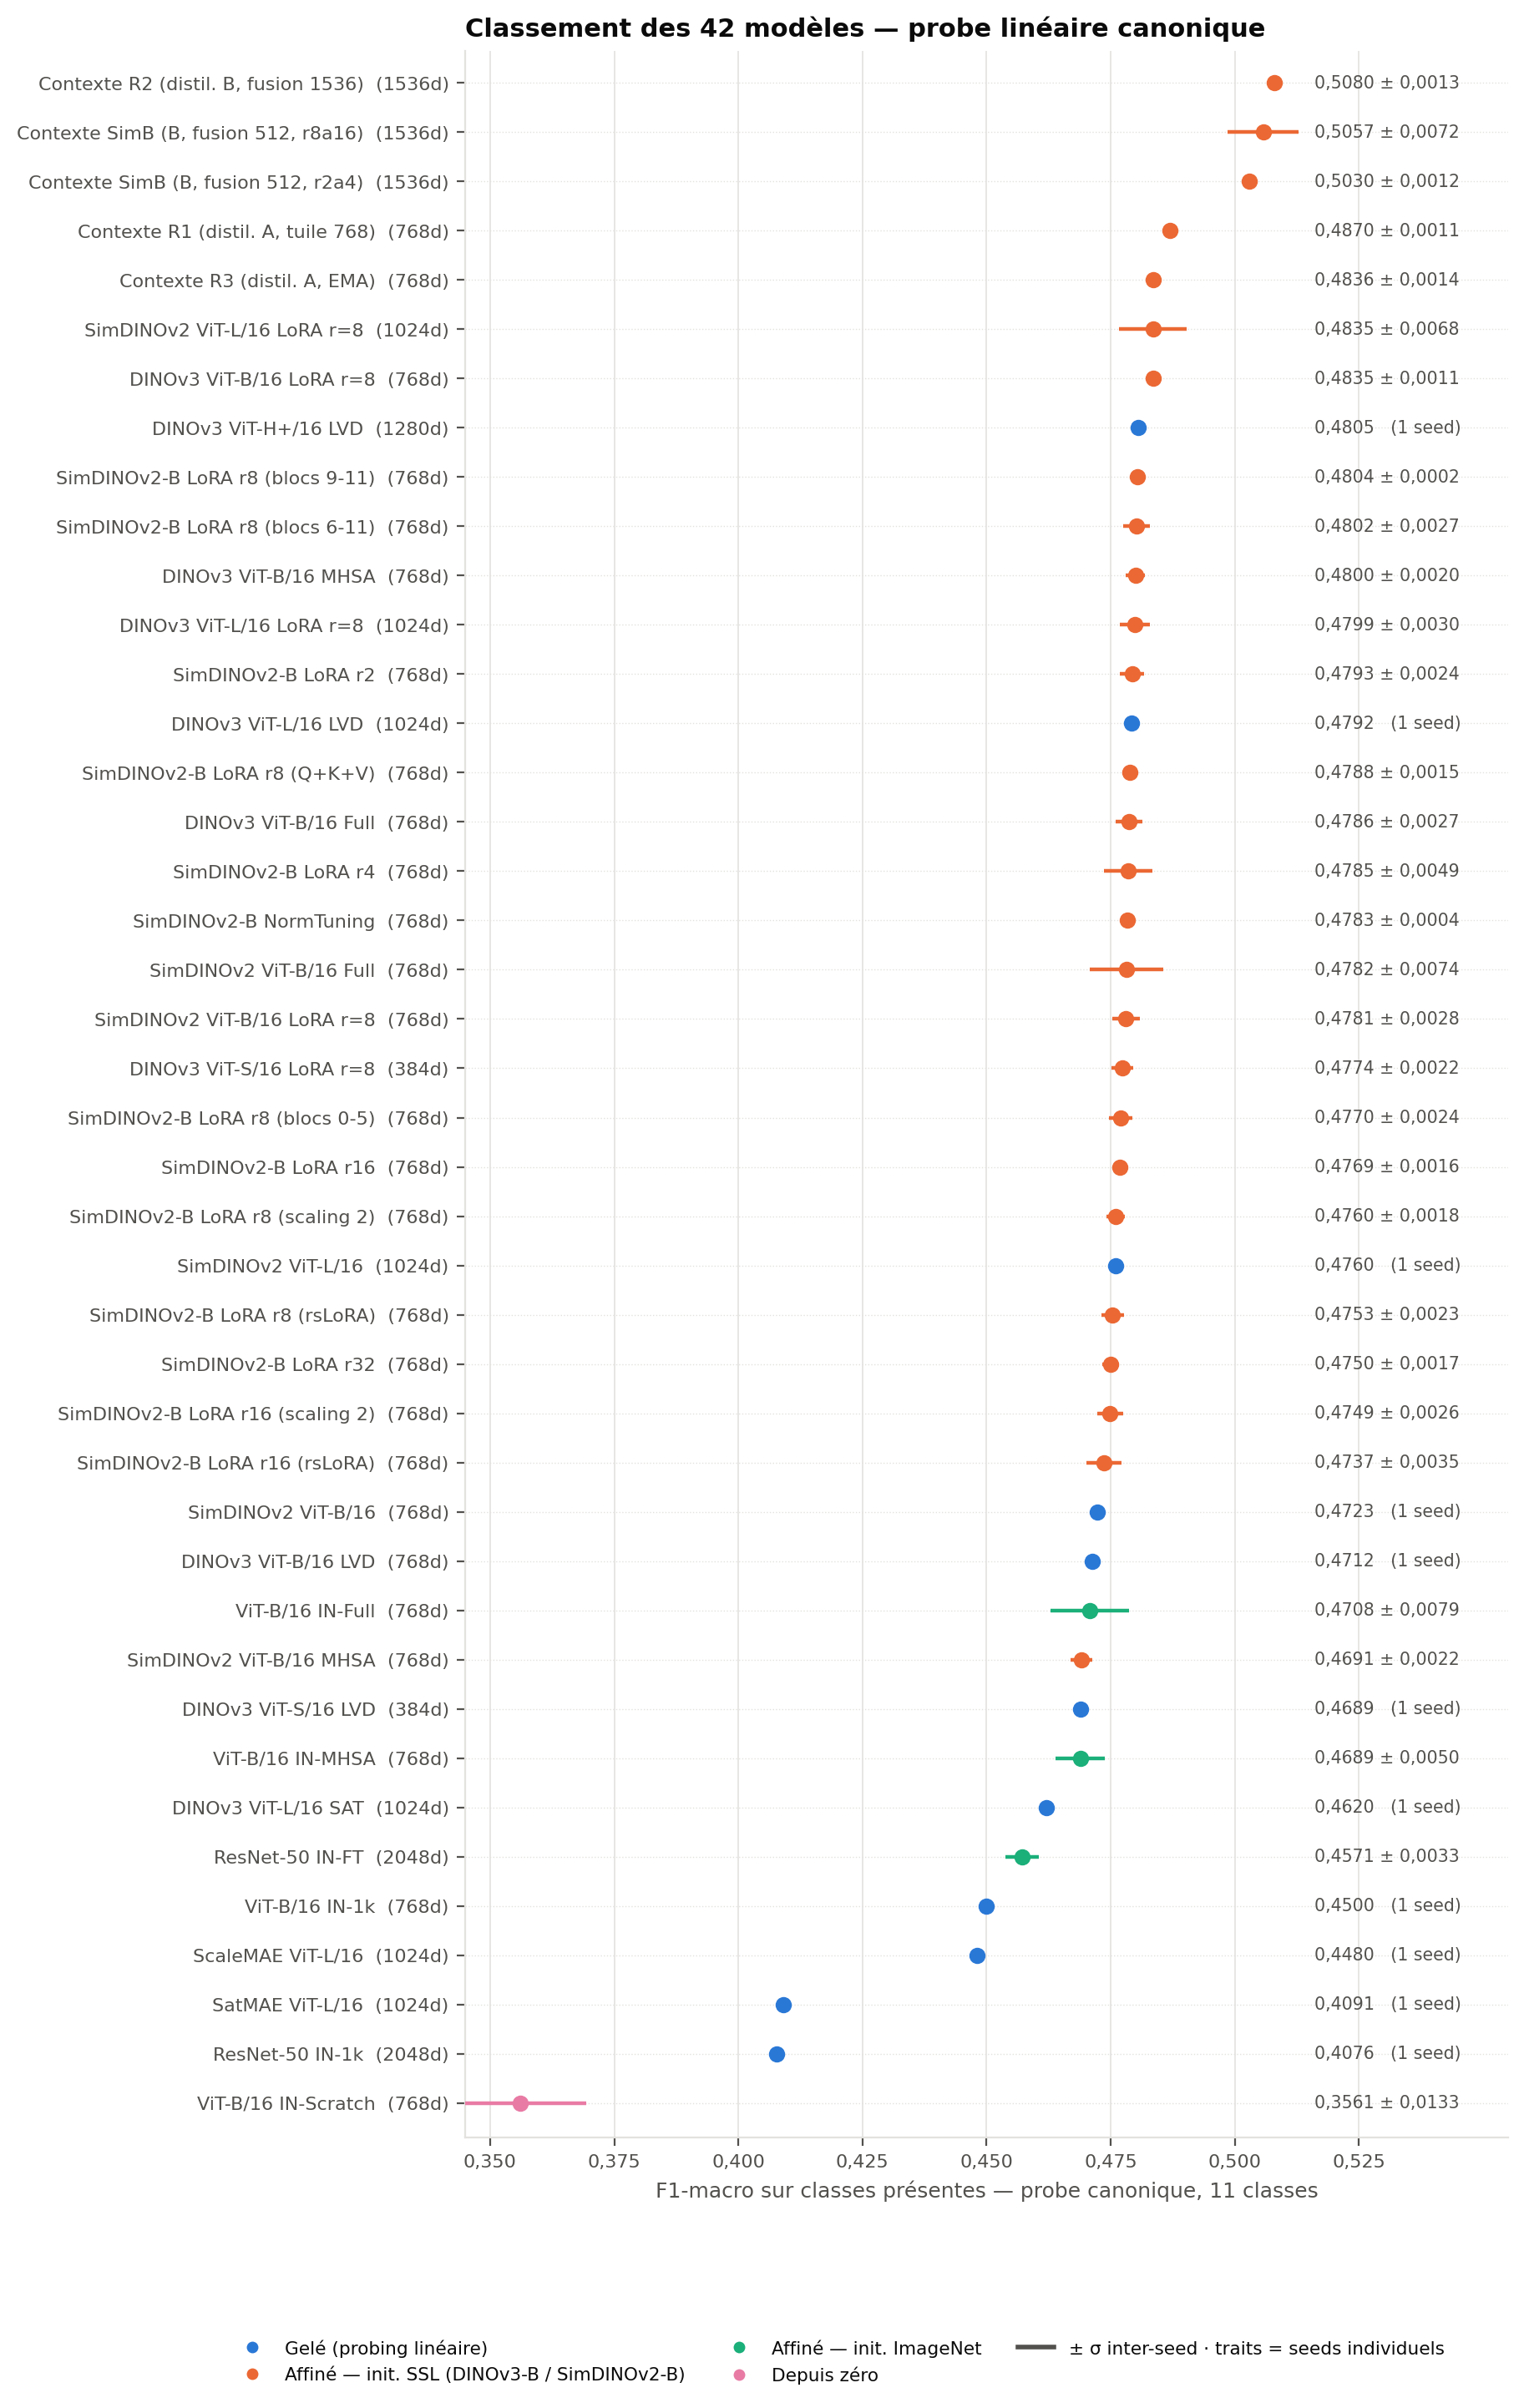
\includegraphics[width=0.95\textwidth]{figures/fig_ranking_ci.png}
	\caption{Classement du palier par F1-macro (schéma 11~classes), barres = IC95 bootstrap apparié. Tête détachée (borne fusionnée R2, non déployable) puis ventre mou : une douzaine de régimes d'adaptation tiennent dans 0,01.}
	\label{fig:ranking}
\end{figure}

\begin{table}[H]
	\centering
	\small
	\caption{F1-macro (\fmpres{}, 11~classes) du haut du palier, probe canonique 3~\emph{seeds} (gelés : seed unique). R2 et SimB-B sont des bornes fusionnées non déployables (contexte requis à l'inférence).}
	\label{tab:master}
	\begin{tabular}{llrr}
		\toprule
		\textbf{Modèle} & \textbf{Régime} & \textbf{F1-macro} & $\sigma$ \\
		\midrule
		R2 Contexte B (fusion 1536) & borne fusionnée & 0,5080 & 0,0013 \\
		SimB Contexte B (fusion 512, r8a16) & borne fusionnée & 0,5057 & 0,0072 \\
		SimB Contexte B (fusion 512, r2a4) & borne fusionnée & 0,5030 & 0,0012 \\
		DINOv3-B LoRA r=8 & LoRA & 0,4835 & 0,0011 \\
		SimL LoRA r=8 & LoRA & 0,4835 & 0,0068 \\
		DINOv3-H+/16 & frozen & 0,4805 & --- \\
		SimB LoRA r8 (blocs 9-11) & LoRA partiel & 0,4804 & 0,0002 \\
		DINOv3-B MHSA & MHSA & 0,4800 & 0,0020 \\
		DINOv3-L LoRA r=8 & LoRA & 0,4799 & 0,0030 \\
		DINOv3-L & frozen & 0,4792 & --- \\
		DINOv3-B Full & Full & 0,4786 & 0,0027 \\
		SimB NormTuning & normes+tête & 0,4783 & 0,0004 \\
		DINOv3-S LoRA r=8 & LoRA & 0,4774 & 0,0022 \\
		SimL & frozen & 0,4760 & --- \\
		SimB & frozen & 0,4723 & --- \\
		DINOv3-B & frozen & 0,4712 & --- \\
		\bottomrule
	\end{tabular}
\end{table}

\subsection{À architecture égale, l'avantage du frozen vient de l'échelle, pas de l'absence d'adaptation}

La comparaison au Tableau~\ref{tab:master} masque un effet de confusion : les meilleurs modèles figés (DINOv3 ViT-L/16, ViT-H+/16) sont plus grands que les backbones affinés de référence (ViT-B). À architecture strictement égale (DINOv3 ViT-B/16), le gelé (F1$=0{,}4712$) sous-performe tous les régimes affinés : LoRA r=8 ($\Delta=+0{,}0114$, $p=0{,}0012$, rejeté BH), MHSA ($\Delta=+0{,}0085$, $p=0{,}016$, non rejeté sur 528~paires) et Full ($\Delta=+0{,}0072$, $p=0{,}101$). Autrement dit, l'affinage supervisé améliore bien la représentation à taille de modèle fixée — le plafond global tient à ce que les meilleurs gelés disponibles bénéficient d'une échelle supérieure, et non à une supériorité intrinsèque du régime figé sur l'affinage.

\subsection{Deux backbones, deux vitesses d'adaptation}
\label{sec:datacurve}

La Figure~\ref{fig:curve} sépare les deux familles : les trois régimes ImageNet dépassent leur gelé (0,4500) dès $\approx$~2\,060~tuiles et plafonnent +0,025 à +0,028 au-dessus, tandis que LoRA met $\approx$~4\,592~tuiles à simplement égaler son gelé DINOv3-B (0,4712) et finit à peine +0,012 — l'adaptation \emph{coûte cher en données} sur un bon pré-entraînement, et rapporte \emph{peu}. À volume égal, LoRA bat toutefois le probing gelé du même backbone à \emph{toutes} les fractions ($\Delta$ de +0,005 à +0,023, maximal à 5\,\%) : la comparaison usuelle « LoRA à $x$\,\% contre gelé à 100\,\% » est une autre question. L'entraînement depuis zéro reste très en-deçà même à 100\,\% (0,355), illustrant la valeur du pré-entraînement même avec des données d'affinage.

\begin{figure}[H]
	\centering
	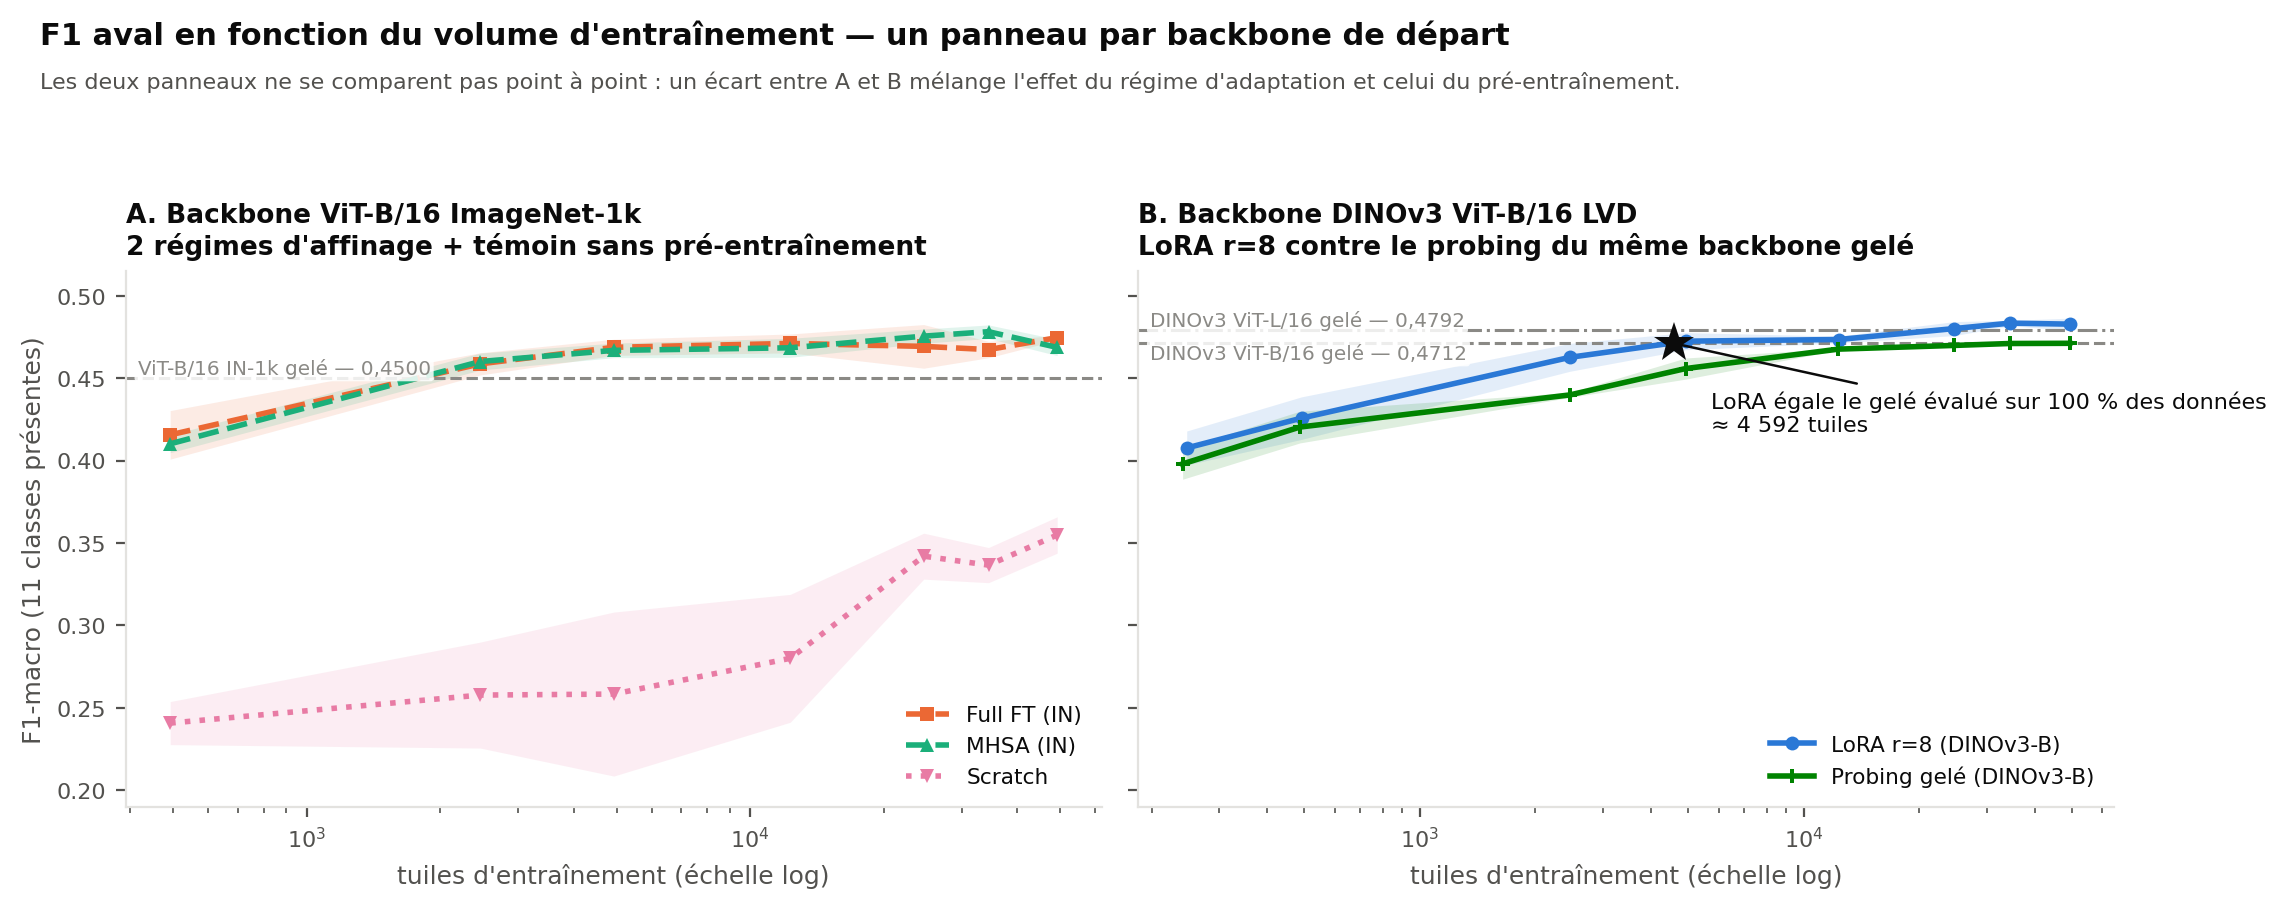
\includegraphics[width=0.95\textwidth]{figures/fig_dc_curves_by_init.png}
	\caption{Courbes de données par backbone (échelle commune). Famille ImageNet : Full/MHSA dépassent leur gelé dès $\approx$~2\,060~tuiles (+0,025 à +0,028 au plafond). Famille DINOv3 : LoRA r=8 égale son gelé vers $\approx$~4\,592~tuiles, finit +0,012. Bandes = $\pm\sigma$ (3~\emph{seeds}).}
	\label{fig:curve}
\end{figure}

\subsection{Le tirage aléatoire surestime : la courbe spatiale}
\label{sec:spatial_curve}

La courbe ci-dessus tire les tuiles au hasard, donc des voisines corrélées entre train et test. La courbe \textbf{spatiale} (blocs contigus sous 25\,\%, orthomosaïques entières au-delà, LoRA r=8 DINOv3-B) est plus dure — et de plus en plus dure avec le volume : à 1\,\%, le F1 spatial vaut 0,099 contre 0,426 en aléatoire ; le plateau est décalé à 50--75\,\% du volume contre $\approx$~5\,\% en aléatoire, et les deux convergent à 100\,\% (0,483). Autrement dit, les courbes usuelles surestiment la performance déployable, surtout à petit volume.

\begin{figure}[H]
	\centering
	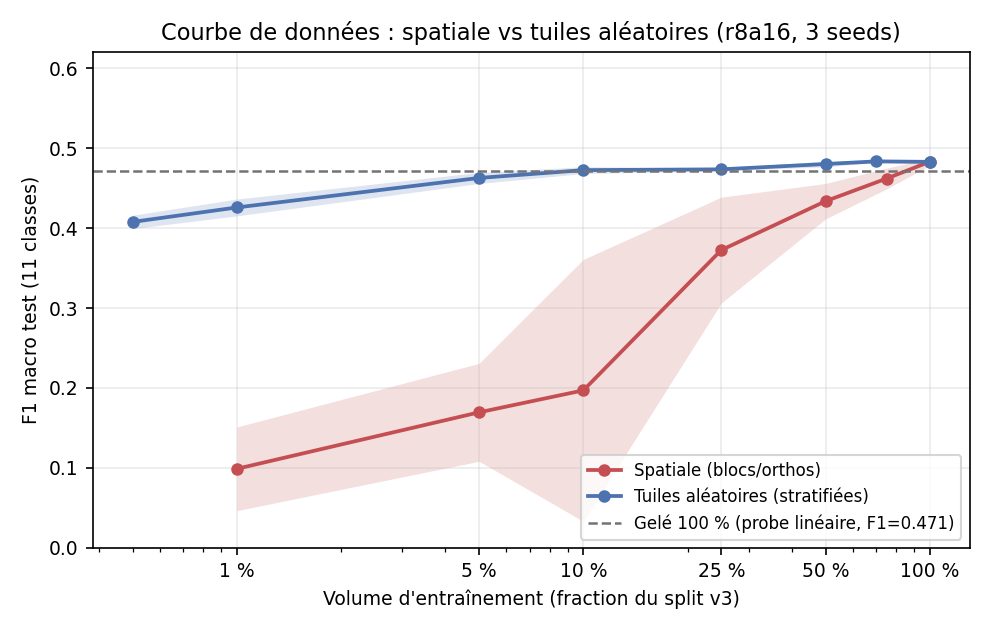
\includegraphics[width=0.8\textwidth]{figures/fig_spatial_vs_random.png}
	\caption{Courbe spatiale vs aléatoire (LoRA r=8, DINOv3-B, 11~classes). Le split spatial est plus dur, et l'écart se creuse avec les données : il évalue ce qui compte vraiment.}
	\label{fig:spatial}
\end{figure}

\subsection{Les modèles de fondation satellite transfèrent mal vers l'imagerie UAV}

Les modèles pré-entraînés spécifiquement sur imagerie satellite sous-performent nettement les modèles génuinistes et bio-spécialisés sur cette tâche UAV~: SatMAE ViT-L/16 (F1$=0.4091$) et Scale-MAE ViT-L/16 (F1$=0.4480$) se classent parmi les derniers du Tableau~\ref{tab:master}, et même DINOv3 ViT-L/16 dans sa variante pré-entraînée SAT-493M (F1$=0.4620$) reste en retrait par rapport à sa contrepartie génuiniste LVD (F1$=0.4792$) et par rapport au meilleur modèle bio-spécialisé (SimDINOv2 ViT-L/16, F1$=0.4760$). Ce constat, cohérent à travers trois architectures et deux stratégies de pré-entraînement satellite distinctes (MAE et DINOv3 continué), documente empiriquement un fossé satellite-vers-drone~: le décalage d'échelle spatiale entre pré-entraînement (10~m à 30~cm/pixel) et évaluation (2.2~mm/pixel) dégrade la qualité de la représentation transférée, malgré la similarité superficielle du domaine (imagerie aérienne de couvert végétal).

\subsection{Le paysage de l'adaptation est plat}
\label{sec:peft_results}

Treize bras $\times$ 3~\emph{seeds} sur SimDINOv2-B (Tableau~\ref{tab:simb}), même test, probe canonique : \textbf{tout tient dans 0,0068} de F1, et aucun écart ancre-vs-bras ne survit au bootstrap apparié ($p=0{,}44$--$0{,}94$). Le rang trace une pente douce décroissante (r2 : 0,4793 $\to$ r32 : 0,4750), sans falaise ; le scaling dégrade monotonement aux deux rangs testés (r8 : 0,4781 $\to$ 0,4760 $\to$ 0,4753 ; r16 : 0,4769 $\to$ 0,4749 $\to$ 0,4737), infirmant rsLoRA~\autocite{kalajdzievski2023rslora} sur ces données — et établissant que le décrochage r16/32 observé sur DINOv3-B est un effet de rang réel, pas un artefact de scaling. L'ordre de position se transpose (blocs hauts $\geq$ tous blocs $\gg$ blocs bas), avec b911 (3~derniers blocs) le plus stable du job ($\pm$0,0002). Le résultat structurel : \textbf{NormTuning (normes + tête, $\approx$47k paramètres) égale LoRA r=8 au millième près} (0,4783 vs 0,4781, $p=0{,}94$) — l'adaptation de ce backbone vaut ce que vaut une mise à jour des normes.

\begin{figure}[H]
	\centering
	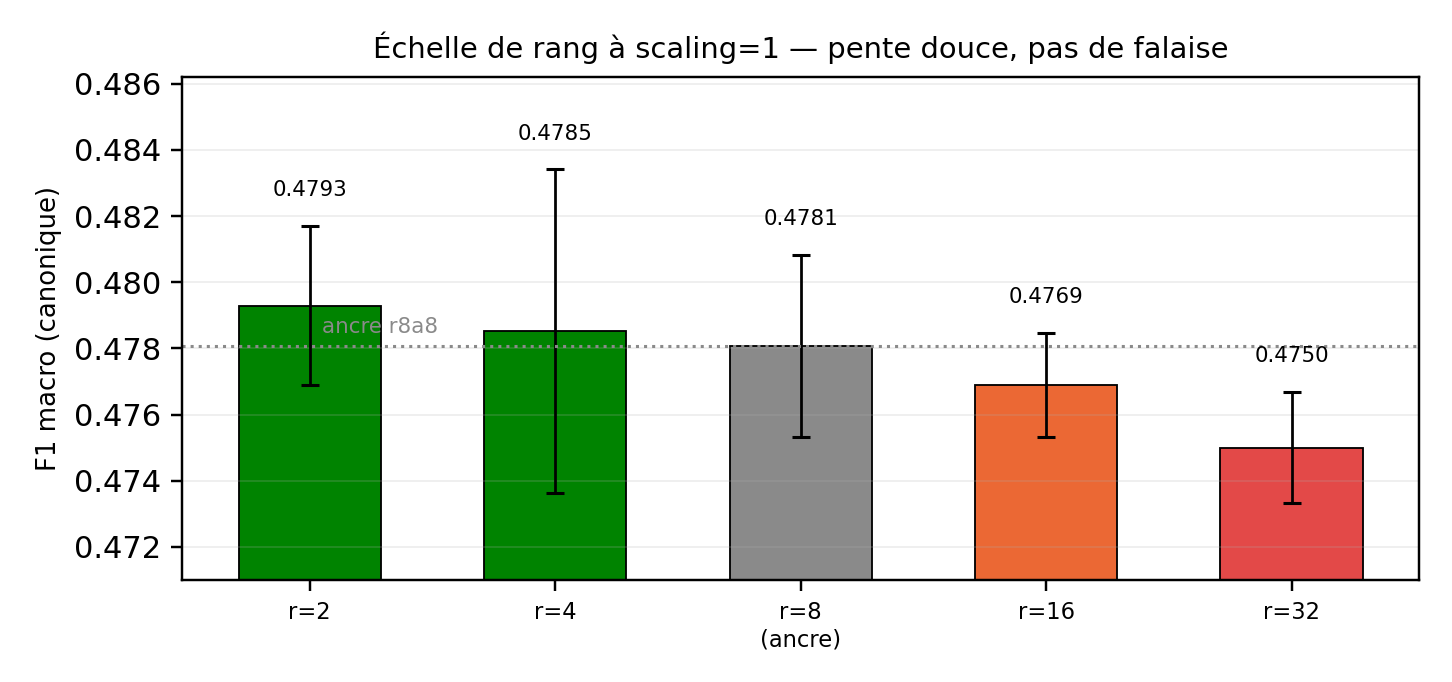
\includegraphics[width=0.72\textwidth]{figures/fig_peft_rank_ladder.png}
	\caption{Ablation du rang LoRA (SimDINOv2-B, scaling=1) : pente douce, sous le seuil d'interprétabilité entre voisins. Le rang 8 est sur un plateau, pas à un optimum.}
	\label{fig:peft_rank}
\end{figure}

\begin{table}[H]
	\centering
	\small
	\caption{Ablation LoRA/PEFT, SimDINOv2-B (tuile seule, F1 canonique). Ancre : r8a8 tous blocs Q/V (0,4781). Aucun bras ne dépasse l'ancre au-delà du bruit.}
	\label{tab:simb}
	\begin{tabular}{lrrr}
		\toprule
		\textbf{Bras} & \textbf{F1} & $\sigma$ & \textbf{Params} \\
		\midrule
		r8, blocs 9-11 & 0,4804 & 0,0002 & 74k \\
		r8, blocs 6-11 & 0,4802 & 0,0027 & 147k \\
		r2, tous blocs & 0,4793 & 0,0024 & 74k \\
		r8, Q+K+V & 0,4788 & 0,0015 & 442k \\
		r4, tous blocs & 0,4785 & 0,0049 & 147k \\
		NormTuning & 0,4783 & 0,0004 & 47k \\
		r8a8 tous blocs (ancre) & 0,4781 & 0,0028 & 295k \\
		r8, blocs 0-5 & 0,4770 & 0,0024 & 147k \\
		r16, tous blocs & 0,4769 & 0,0016 & 590k \\
		r8 scaling 2 / rsLoRA & 0,4760 / 0,4753 & 0,0018 / 0,0023 & 295k \\
		r32, tous blocs & 0,4750 & 0,0017 & 1\,180k \\
		r16 scaling 2 / rsLoRA & 0,4749 / 0,4737 & 0,0026 / 0,0035 & 590k \\
		gelé & 0,4723 & --- & 0 \\
		\bottomrule
	\end{tabular}
\end{table}

\subsection{Le contexte spatial déplace le plafond}
\label{sec:context_results}

La fusion [tuile~;~voisinage 512~px] apporte +0,025 à +0,034 (Tableau~\ref{tab:ctx}) : R2 entraîné (design B, DINOv3-B) atteint \textbf{0,5080}, et SimDINOv2-B \textbf{gelé-fusionné} atteint 0,5059 \emph{sans aucun entraînement} — quand toute l'ablation PEFT tient dans 0,0068. La distillation seule (design A, 0,4870) ne bat pas les baselines LoRA : le gain exige la fusion apprise (ou pré-alignée). Deux contrôles isolent le spatial : contexte seul = tuile seule (0,4780 vs 0,4779), contexte permuté \emph{sous} la tuile seule (0,4745) — une seconde représentation désalignée nuit. Le sweep gelé (5~backbones $\times$ 3~tailles) confirme 512 $>$ 1024 $\gg$ 2048 partout, en ligne avec Gomes et al.~\autocite{gomes2026efficient} ; SimL (300M) n'ajoute rien sur SimB (0,5022 vs 0,5059) : c'est l'alignement iNat-Plantae qui décode le voisinage, pas la taille. Et l'affinage complet n'apporte rien sur SimB entraîné (0,5057 $\approx$ gelé-fusionné 0,5059). R2 reste une borne non déployable (contexte requis à l'inférence), qui sacrifie sa représentation tuile-seule (0,4779, pire que R1) pour la fusion.

\begin{figure}[H]
	\centering
	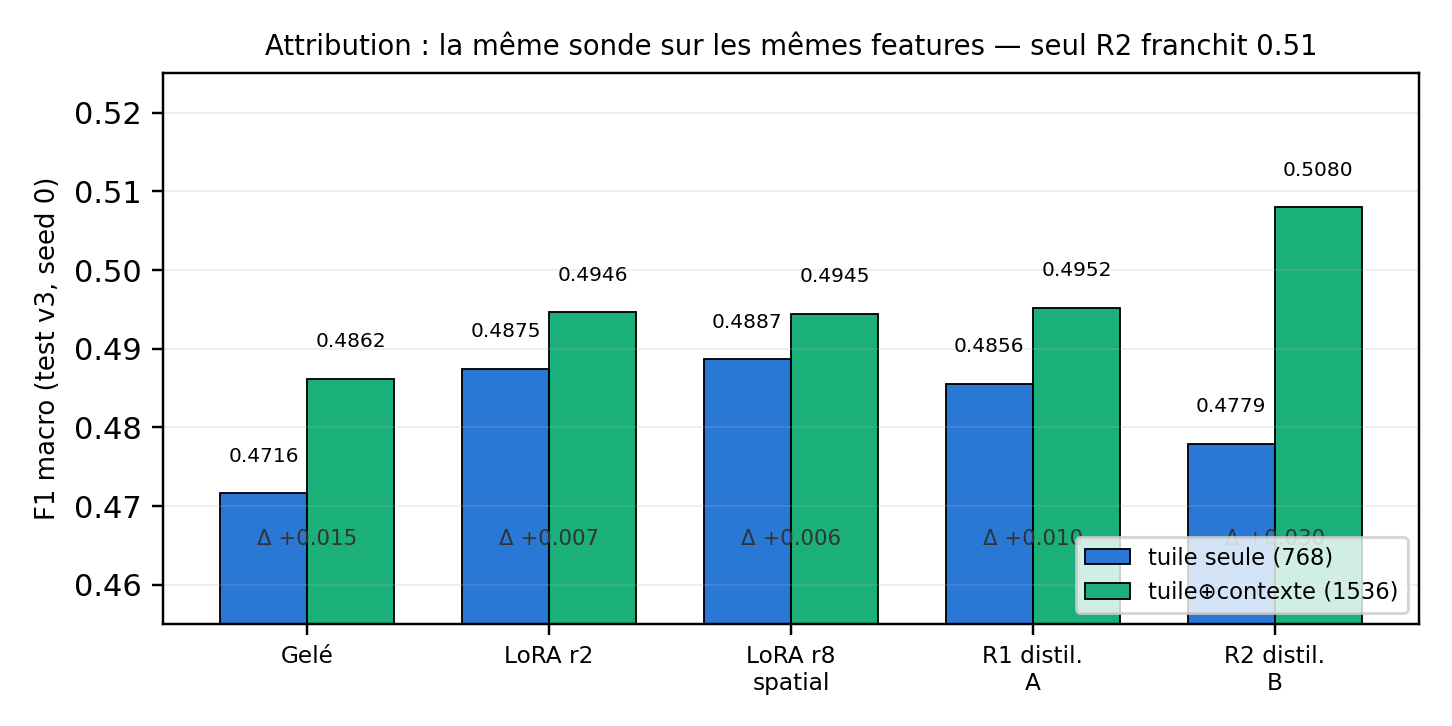
\includegraphics[width=0.72\textwidth]{figures/fig_ctx_matrix.png}
	\caption{Le contexte aide tous les modèles ; seul R2 (fusion apprise) franchit 0,51, au prix d'une tuile seule dégradée.}
	\label{fig:ctx}
\end{figure}

\begin{table}[H]
	\centering
	\small
	\caption{Contexte : designs et sweep gelé (sélection). F1-macro 11~classes, test v3.}
	\label{tab:ctx}
	\begin{tabular}{llr}
		\toprule
		\textbf{Configuration} & \textbf{Détail} & \textbf{F1} \\
		\midrule
		R2 design B (entraîné) & DINOv3-B, fusion apprise & 0,5080 $\pm$ 0,0015 \\
		SimB gelé-fusionné @512 & sonde seule, 0 entraînement & 0,5059 \\
		SimB entraîné B @512 (r8a16) & LoRA + distillation + tête & 0,5057 $\pm$ 0,0072 \\
		R1 design A (distillation seule) & tuile seule à l'inférence & 0,4870 $\pm$ 0,0011 \\
		DINOv3-B gelé-fusionné @512 & sonde seule & 0,4953 \\
		tuile seule / contexte seul / permuté & contrôles R2 & 0,4779 / 0,4780 / 0,4745 \\
		\bottomrule
	\end{tabular}
\end{table}

\subsection{La séparabilité ordonne, le spectre non}
\label{sec:latent}

La Figure~\ref{fig:scatter} met en relation le score de silhouette (espace latent figé, sans affinage ni supervision) et le F1 aval. Sur trois populations emboîtées (40~modèles, 11~gelés, palier de 35), le verdict dépend de la puissance : à $n=12$, seule la silhouette paraissait robuste ; à $n=35$, \textbf{toute la famille séparabilité passe la correction BH par famille} (Tableau~\ref{tab:tier} : Fisher 69\,\%, DBI/CHI/NC1 67\,\%, silhouette 64\,\%, $p_{BH}\leq0{,}046$), tandis que la famille spectrale ordonne \textbf{à l'envers} (41--42\,\%). Sa corrélation d'ensemble positive n'est portée que par les modèles cassés. Seule la pureté k-NN désigne le vrai n\textsuperscript{o}~1 (R2).

\begin{figure}[H]
	\centering
	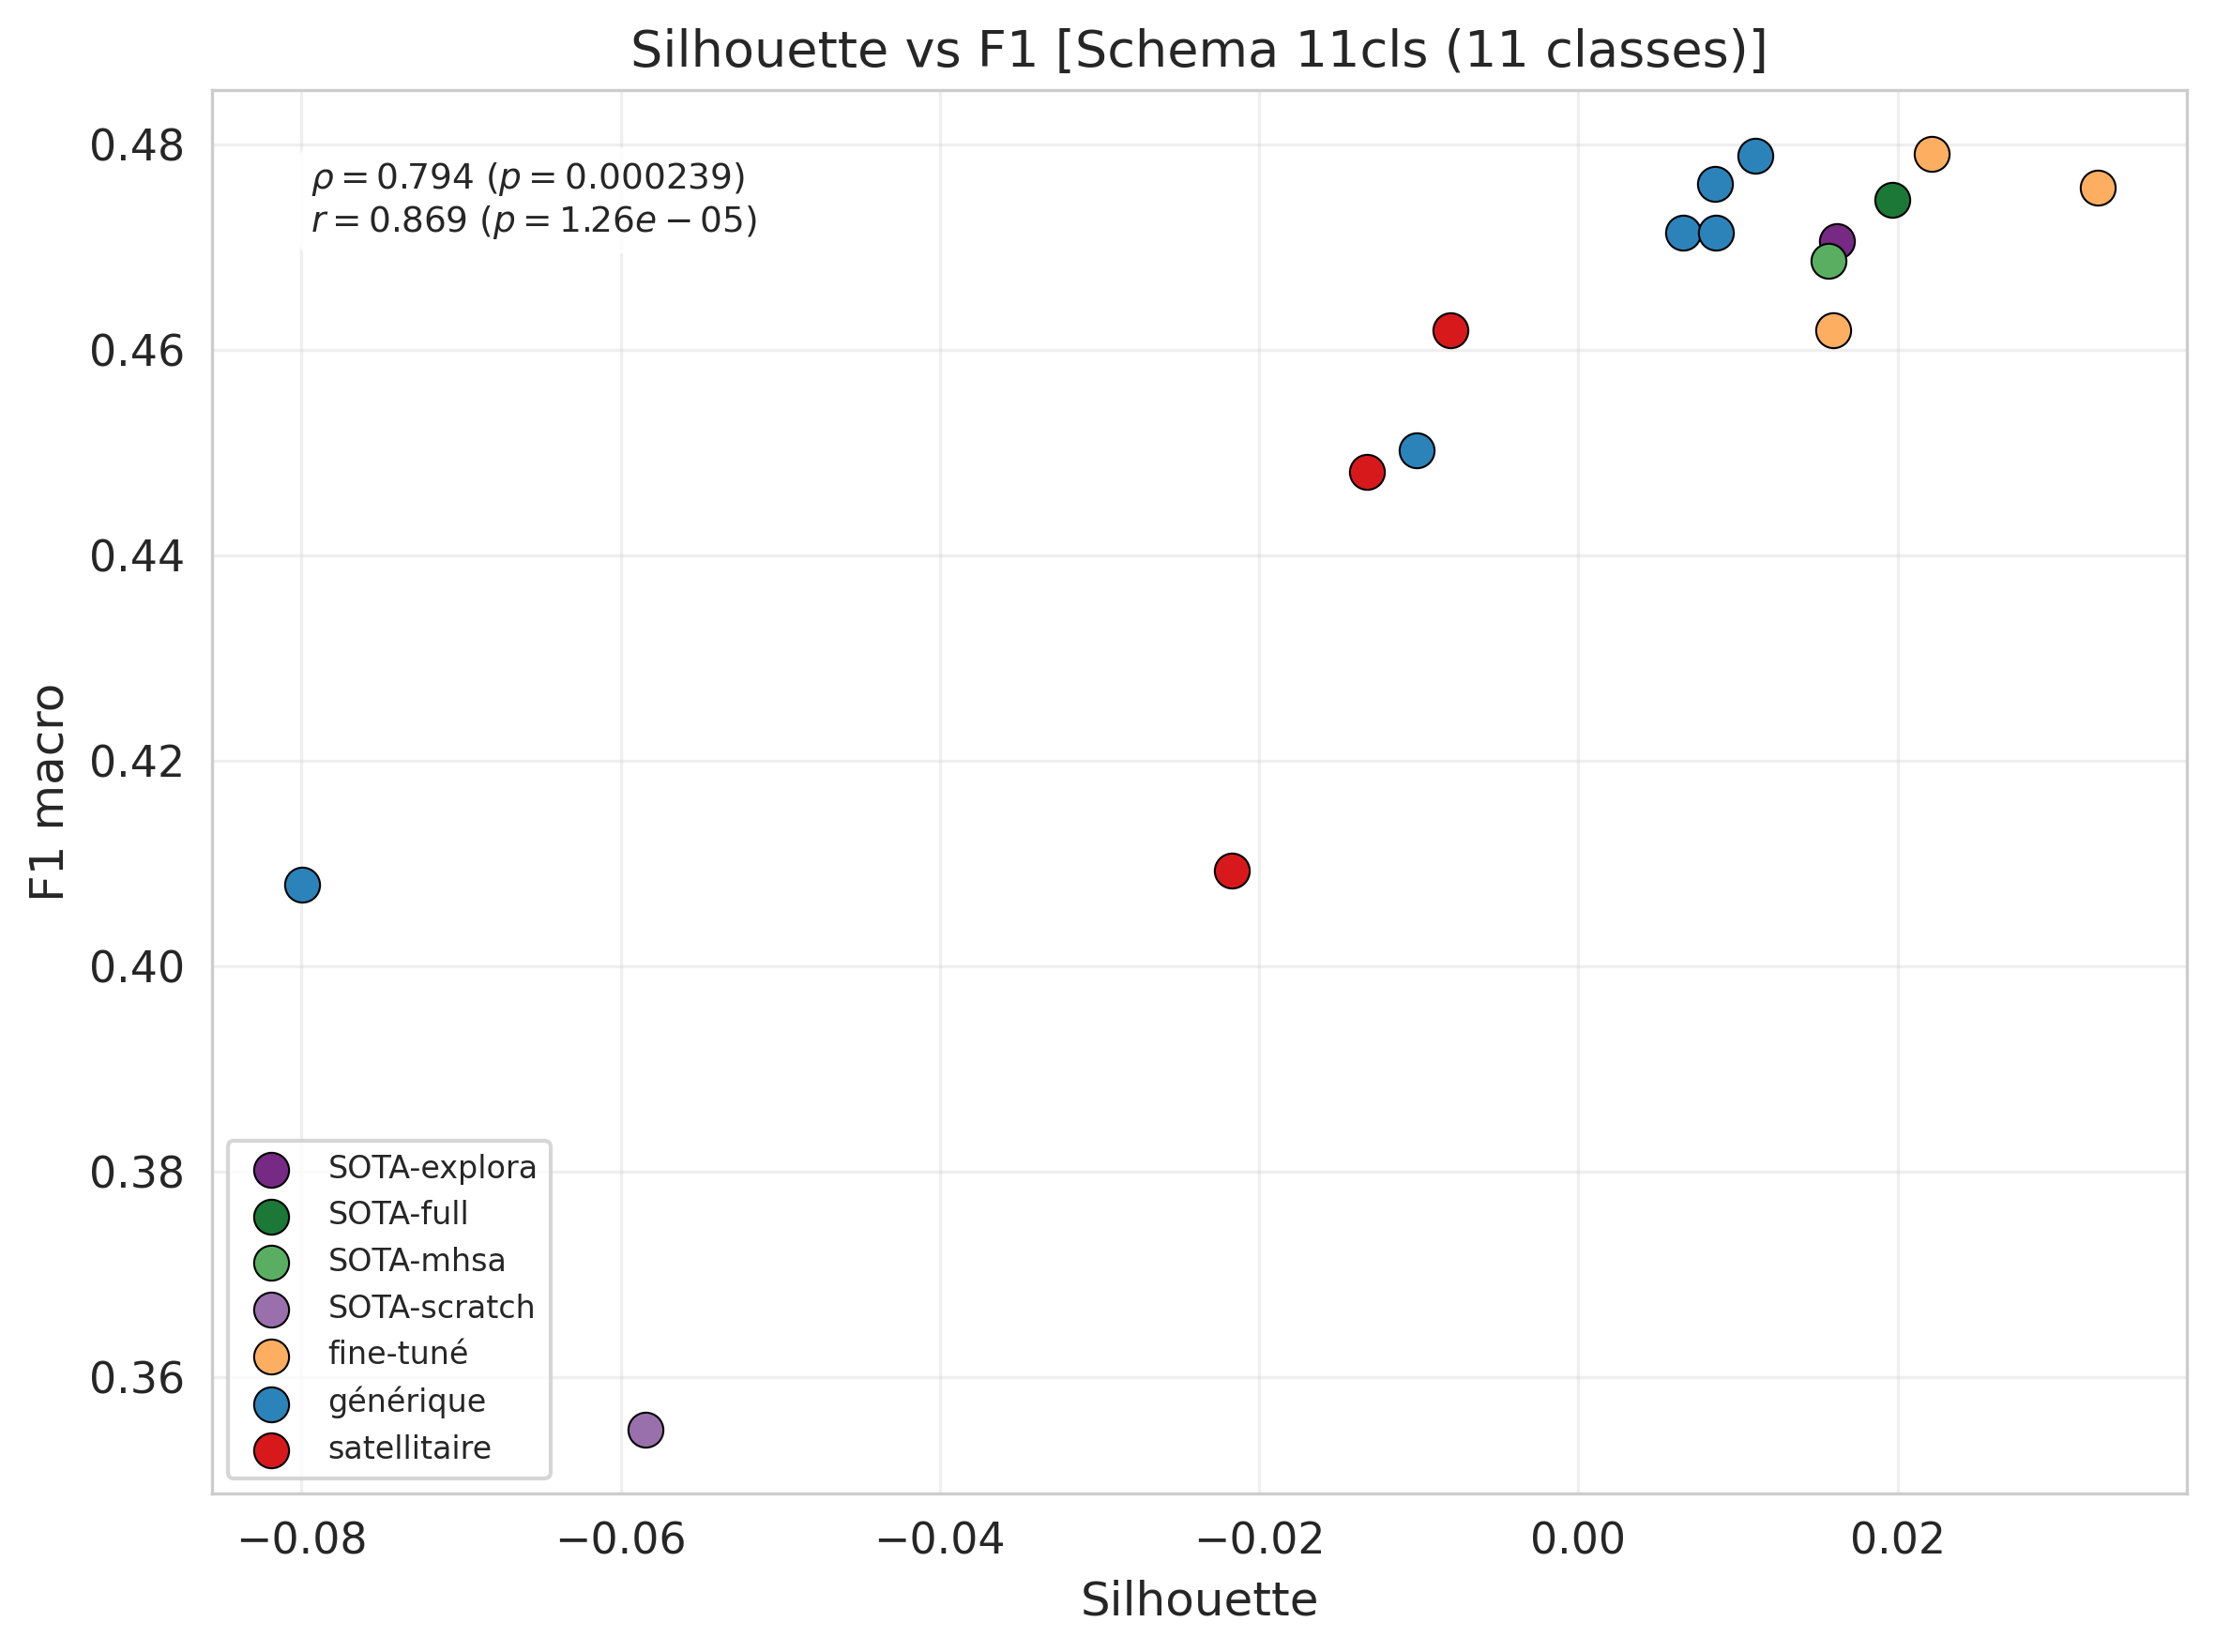
\includegraphics[width=0.75\textwidth]{figures/fig3_scatter_silhouette_f1.png}
	\caption{Silhouette (figé, sans supervision) vs F1 aval. La relation est tirée par les modèles faibles ; dans le palier, c'est toute la famille séparabilité qui ordonne.}
	\label{fig:scatter}
\end{figure}

\begin{table}[H]
	\centering
	\small
	\caption{Pouvoir d'ordonnancement sur le palier de 35 (592~paires ; hasard = 296). $p_{BH}$ corrigé par famille pré-déclarée. Seule la pureté k-NN désigne le vrai meilleur modèle.}
	\label{tab:tier}
	\begin{tabular}{lrrrr}
		\toprule
		\textbf{Métrique} & \textbf{Paires} & \% & $\rho$ & $p_{BH}$ \\
		\midrule
		Ratio de Fisher & 411/592 & 69 & +0,48 & 0,013 \\
		Davies-Bouldin & 399/592 & 67 & -0,43 & 0,039 \\
		Calinski-Harabasz & 396/592 & 67 & +0,43 & 0,014 \\
		NC1 & 396/592 & 67 & -0,43 & 0,014 \\
		Silhouette & 376/592 & 64 & +0,38 & 0,026 \\
		Pureté k-NN & 342/592 & 58 & +0,25 & 0,203 \\
		LogME (test) & 330/592 & 56 & +0,12 & 0,961 \\
		Rang effectif & 240/592 & 41 & -0,24 & 0,341 \\
		\bottomrule
	\end{tabular}
\end{table}

Ce résultat suggère un protocole de présélection à faible coût (silhouette ou Fisher sur embeddings figés avant toute évaluation supervisée), sous réserve d'une validation \emph{leave-one-model-out} et d'un test sur un second jeu de données (\S\ref{sec:discussion}).

\paragraph{Combien de dimensions la tâche utilise-t-elle ?} Une explication candidate du fait que le rang effectif ordonne à l'envers est que la tâche ne dépend que d'un petit sous-espace des dimensions de l'embedding. Une sonde tronquée par analyse en composantes principales sur DINOv3-B LVD (Tableau~\ref{tab:dimprobe}) confirme cette lecture~: $k=50$ composantes suffisent déjà à atteindre 98,2\,\% du F1 obtenu avec les 768 dimensions, et $k=100$ en atteint 99,1\,\%~; les 668 dimensions restantes n'apportent que $+0{,}004$. La tâche vit donc dans un sous-espace d'environ 100 dimensions, ce qui explique à la fois pourquoi le rang effectif (mesure globale) ne prédit pas le F1 et pourquoi la géométrie \emph{globale} — isotropie, rang — n'est pas le bon levier~: c'est le contenu informationnel des directions utiles qui compte, pas le nombre de directions occupées.

\begin{table}[H]
	\centering
	\small
	\caption{Sonde tronquée par PCA sur DINOv3-B LVD gelé~: F1 test de la sonde canonique selon le nombre $k$ de composantes principales conservées (test 17\,598~tuiles).}
	\label{tab:dimprobe}
	\begin{tabular}{lrrrrrrr}
		\toprule
		$k$ & 10 & 20 & 50 & 100 & 200 & 400 & 768 \\
		\midrule
		F1 test & 0,408 & 0,446 & 0,463 & 0,467 & 0,467 & 0,469 & 0,472 \\
		\% du plein & 86,6 & 94,7 & 98,2 & 99,1 & 99,1 & 99,5 & 100 \\
		\bottomrule
	\end{tabular}
\end{table}

\subsection{Coût, déploiement et classes apprenables}
\label{sec:cost}

Pour le praticien, le F1 ne suffit pas. DINOv3-B LoRA r=8 atteint 0,4835 à \textbf{82~ms/image sur CPU} (quasi temps réel), quand R2 (0,5080) coûte 675~GFLOPs (tuile$\oplus$contexte) contre 17,6 pour la tuile seule — et que DINOv3-H+ gelé (0,4805, 840M params) exige une GPU pour un F1 moindre : à budget fixé, l'adaptation est l'option efficace, et le contexte l'option puissante mais coûteuse. Par classe, ARCA/DRYI/RUBC restent à F1~$\approx$~0 pour \emph{tous} les modèles et toutes les fractions : sous $\sim$200~tuiles de test, c'est le jeu test — pas le modèle — qui décide quelles classes sont apprenables. Le probe linéaire bat le meilleur k-NN partout et de loin.

\begin{figure}[H]
	\centering
	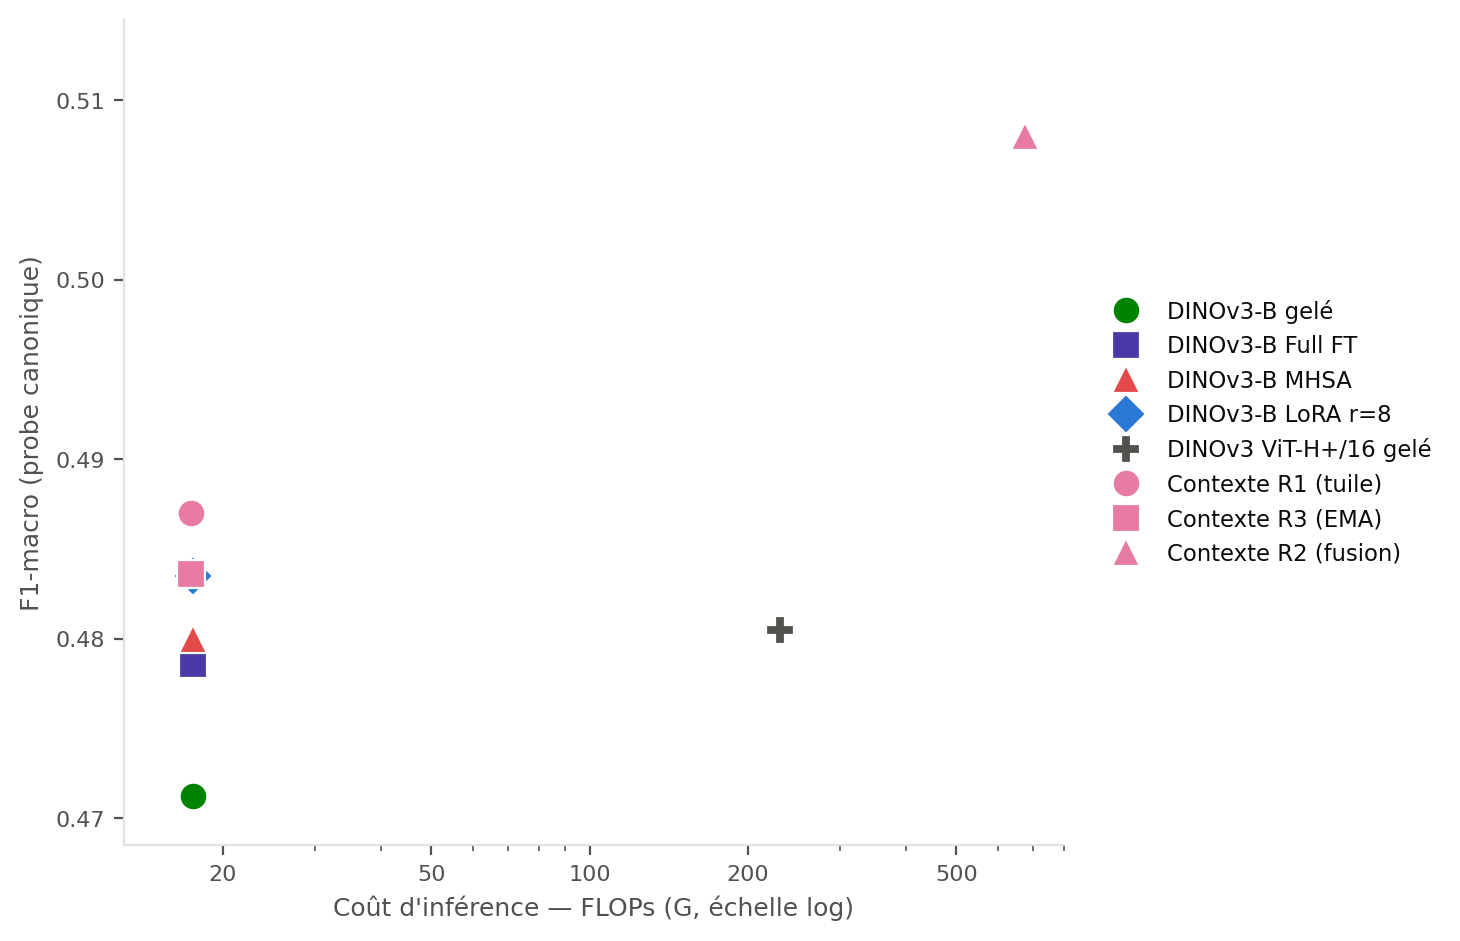
\includegraphics[width=0.82\textwidth]{figures/fig_cost_perf.png}
	\caption{F1 vs coût d'inférence (échelle log). R2 est le meilleur mais le plus coûteux ; LoRA r=8 domine le compromis déployable.}
	\label{fig:cost}
\end{figure}

\subsection{Analyse layerwise (DINOv3 ViT-L/16)}

Une analyse complémentaire de la géométrie latente couche par couche (24~couches, DINOv3 ViT-L/16, variantes LVD et SAT) est fournie en annexe. Un F1 par couche n'est disponible que pour ViT-B/16 ImageNet (12~couches), pour lequel les corrélations intra-modèle (\emph{within-model}) entre géométrie et F1 divergent des corrélations inter-modèles (Tableau~\ref{tab:tier} : le rang effectif inter-modèles ordonne à l'envers sur le palier) --- une divergence attribuable à deux facteurs : (i)~un confondant de dimension (le rang effectif compare des embeddings de dimensions différentes en inter-modèles --- 768 pour ViT-B, 1024 pour ViT-L, 2048 pour ResNet-50 --- alors qu'en intra-modèle la dimension est constante) ; (ii)~une unité d'analyse différente (sélectionner une couche n'est pas le même problème que sélectionner un modèle)~: Spearman(RankMe normalisé, F1)$=0.825$ et Spearman(anisotropie, F1)$=-0.881$ (n=12~couches). Ces corrélations intra-modèle ne constituent cependant pas une preuve de généralisation, étant calculées sur un seul modèle ; le F1 par couche pour DINOv3 ViT-L/16 reste indisponible faute d'accès aux embeddings layerwise complets sur le cluster de calcul.

%==========================================================================
\section{Discussion}
\label{sec:discussion}
%==========================================================================

\subsection{Ce que signifie « l'adaptation est bornée »}

Le résultat central — aucun modèle déployable (tuile seule) ne dépassant significativement le meilleur gelé, alors même que LoRA r=8 bat son propre backbone de +0,0114 ($p=0{,}0012$) — ne doit pas être lu comme « l'affinage supervisé est inutile ». À architecture égale, l'affinage améliore significativement la représentation. Le message pratique est plus nuancé~: sur cette tâche et à ce volume de données, \emph{adapter rattrape la capacité, elle ne la dépasse pas}. L'ablation systématique sur SimDINOv2-B (13~bras $\times$ 3~\emph{seeds}, tout dans 0,0067 de F1, aucun écart ancre-vs-bras significatif au bootstrap apparié, $p=0{,}44$--$0{,}94$) précise ce verdict : le paysage de l'adaptation est plat, NormTuning ($\approx$47k paramètres) égale LoRA au millième près, et le scaling LoRA dégrade monotonement (hypothèse rsLoRA infirmée). Pour un praticien en écologie disposant de ressources limitées — le cas typique en cartographie de végétation arctique — un modèle figé de grande échelle \emph{ou} une adaptation parcimonieuse (blocs hauts, petit rang) valent un affinage complet, sans perte mesurable ; seule l'information — le contexte spatial — déplace le plafond.

\subsection{Le contexte spatial : le seul levier qui déplace le plafond}

La fusion [tuile~;~voisinage 512~px] apporte +0,025 à +0,034 de F1 (R2 entraîné : 0,508 ; SimDINOv2-B gelé-fusionné : 0,5059, sans aucun entraînement), quand toute l'ablation PEFT tient dans 0,0067. Deux contrôles valident que ce gain est bien spatial : le contexte seul égale la tuile seule (0,4780 vs 0,4779), et le contexte permuté dégrade sous la tuile seule (0,4745) — une seconde représentation désalignée nuit, seule l'information de voisinage appariée aide. Le sweep multi-backbones confirme le pattern 512~$>$~1024~$\gg$~2048 sur cinq backbones, et l'affinage complet n'apporte rien sur SimB quand le pré-entraînement est aligné (iNat-Plantae). En pratique : à budget fixé, investir dans le voisinage et dans un backbone aligné au domaine rapporte un ordre de grandeur de plus qu'investir dans l'adaptation des poids. La borne fusionnée reste non déployable en l'état (contexte requis à l'inférence) — c'est une borne informationnelle, pas un modèle de terrain.

\subsection{Le fossé satellite-vers-drone et ses implications pour le choix de modèle}

Le sous-transfert systématique des modèles pré-entraînés sur imagerie satellite (SatMAE, Scale-MAE, DINOv3-SAT) confirme, sur une tâche réelle de végétation, un signal déjà documenté au niveau de la géométrie des représentations~\autocite{sosa2024effective}~: la proximité superficielle de domaine (imagerie aérienne de couvert végétal) ne suffit pas à garantir un transfert efficace lorsque l'échelle spatiale du pré-entraînement (résolution décamétrique) diffère de plusieurs ordres de grandeur de celle de la tâche cible (résolution millimétrique). Ceci a une implication directe pour la pratique~: le choix d'un modèle de fondation pour une tâche UAV en écologie ne devrait pas se fonder sur l'étiquette de domaine du pré-entraînement (« modèle géospatial » ou « modèle de télédétection ») mais sur la proximité effective d'échelle spatiale et de statistique d'image entre corpus de pré-entraînement et corpus cible.

\subsection{Le score de silhouette comme outil de triage de modèle}

La corrélation forte et stable de la famille séparabilité avec le F1 aval (\S\ref{sec:latent}) suggère un protocole de présélection à faible coût~: calculer les embeddings figés de plusieurs modèles candidats sur un petit échantillon non annoté (ou faiblement annoté) du domaine cible, en dériver la silhouette ou le ratio de Fisher par rapport à un regroupement grossier (par exemple des \emph{pseudo-classes} obtenues par clustering non supervisé, ou un sous-ensemble d'étiquettes existant), et ne retenir pour un affinage ou une évaluation supervisée complète que les modèles les mieux classés par cette métrique. Un tel protocole réduirait le coût de sélection de modèle, actuellement dominé par l'entraînement et l'évaluation supervisée complète de chaque candidat. Nous soulignons toutefois que cette perspective reste, en l'état de la présente étude, une hypothèse dérivée d'une corrélation \emph{inter-modèles} sur un palier de 35~modèles et deux schémas de classes~: elle nécessiterait, pour être validée comme protocole opérationnel, une évaluation \emph{leave-one-model-out} (entraîner la relation séparabilité-F1 sur $n-1$ modèles et prédire le F1 du modèle exclu) et un test sur un second jeu de données de végétation indépendant, deux validations qui sortent du périmètre du présent travail et constituent une perspective naturelle de suite.

\subsection{Limites méthodologiques}
\label{sec:limits}

\paragraph{Bugs connus et corrigés.} Deux anomalies ont été identifiées et corrigées au cours du projet~: (i)~un scheduler de régularisation figé à $C=0.01$ au lieu du meilleur $C$ canonique dans deux scripts d'évaluation, corrigé avant la production des résultats présentés ici~; (ii)~une cascade de réduction de classes manquante dans le calcul des intervalles de confiance du schéma 8~classes (les classes n'étaient pas réduites avant le nouvel ajustement du probe), corrigée par l'application d'une cascade consciente de la source des annotations. Les résultats 8~classes de cet article utilisent la version corrigée.

\paragraph{\fmall{} contre \fmpres{}.} Le F1-macro « brut » (\fmall{}), incluant les classes structurellement non évaluables (RHOL absente du test, ARCA/DRYI/RUBC quasi absentes), biaise la moyenne macro vers le bas de façon non informative sur la qualité réelle des modèles. Cet article cite exclusivement \fmpres{}, restreint aux classes présentes et raisonnablement représentées dans le split de test, choix documenté et cohérent à travers toutes les analyses.

\paragraph{Lacunes de couverture.} Le bootstrap complet (IC95, 528~paires) couvre le palier compétitif de 35~modèles mais pas l'ensemble des configurations de la courbe de données (\S\ref{sec:sota_methods}), qui ne rapporte donc que des moyennes et écarts-types sur 3~\emph{seeds}. Le F1 par couche pour DINOv3 ViT-L/16 (24~couches) reste indisponible, seules les métriques géométriques layerwise ayant pu être calculées, en raison de contraintes d'accès disque aux embeddings complets sur le cluster de calcul (Narval). Le corpus de modèles figés reste par ailleurs limité aux architectures ResNet, ViT et à leurs variantes DINOv2/DINOv3/SimDINOv2/MAE~: aucune architecture ConvNeXt, Swin ou autre architecture hybride convolution-attention récente n'a été incluse.

\paragraph{Limites du corpus de données.} Arctic-TVC reste un corpus de taille modeste (49\,281~tuiles d'entraînement au maximum, soit environ 69.5\,\% des $\sim$70\,000~tuiles totales disponibles) et fortement déséquilibré (ratio de déséquilibre par comptage $\approx31$, par longueur $\approx275$). Le split respecte une contrainte spatiale stricte par orthomosaïque entière, éliminant toute fuite spatiale directe, mais les 9~orthomosaïques de test ($\sim$21.9\,\% des tuiles) ne couvrent pas nécessairement toute la diversité de terrain présente dans le site d'étude. Enfin, la résolution spatiale (GSD) varie entre orthomosaïques~: 2.2~mm/pixel pour la majorité des missions, mais 8 à 17~mm/pixel pour 4~orthomosaïques de mission dite « paysage », introduisant une hétérogénéité de résolution non contrôlée dans l'évaluation.

\paragraph{Portée géographique et taxonomique.} L'ensemble des résultats est établi sur un site unique (Trail Valley Creek, Territoires du Nord-Ouest) et 12~classes de végétation arctique. La généralisation à d'autres biomes de toundra, d'autres compositions floristiques ou d'autres capteurs UAV (multispectral, hyperspectral) n'est pas évaluée dans ce travail et constitue une direction naturelle de validation externe.

\subsection{Perspectives futures}

Au-delà de la validation \emph{leave-one-model-out} du protocole de triage par silhouette (\S5.3), plusieurs directions découlent directement des limites identifiées~: (i)~compléter le bootstrap d'intervalles de confiance sur l'ensemble de la courbe de données plutôt que sur les 12~modèles canoniques seuls~; (ii)~résoudre la contrainte d'accès disque limitant l'analyse layerwise afin d'obtenir un F1 par couche pour DINOv3 ViT-L/16 et tester si la corrélation géométrie-F1 intra-modèle observée sur ViT-B/16 ImageNet se généralise aux architectures plus profondes et à plus grande échelle~; (iii)~étendre le corpus de modèles figés à des architectures convolutionnelles modernes (ConvNeXt) et à des architectures hybrides, afin de vérifier si le fossé satellite-vers-drone et l'avantage d'échelle observés sont spécifiques à la famille ViT~; (iv)~valider les résultats sur un second site ou biome arctique afin de tester la portée géographique des conclusions.

\paragraph{Ajouter de l'information plutôt que de la capacité.} Nos résultats montrent que le plafond est déplacé par l'information (le contexte spatial, \S\ref{sec:context_results}) et non par la capacité ni par la géométrie globale — la tâche ne mobilise qu'environ 100 dimensions (\S\ref{sec:latent}). Trois sources d'information complémentaires, documentées dans la littérature, méritent d'être testées sur Arctic-TVC. (i)~La \emph{structure topographique}~: la végétation arctique est organisée par la microtopographie (polygones de glace, humidité, drainage), et l'ajout de métriques structurelles issues de LiDAR ou d'un modèle numérique de surface améliore la discrimination des communautés végétales par rapport au RGB seul~\autocite{banerjee2022uavlidar}~; un tel canal peut être dérivé d'une acquisition photogrammétrique, sans nouvelle campagne de terrain. (ii)~L'\emph{information spectrale}~: les canaux proche-infrarouge et \emph{red edge}, absents du RGB, codent la productivité et la composition et améliorent la cartographie de la toundra~\autocite{bhuiyan2020spectral}~; l'imagerie multispectrale embarquée sur drone est une pratique établie pour l'écologie arctique~\autocite{yang2022uas} et la combinaison optimale des bandes reste ouverte. (iii)~Le \emph{signal temporel et la saisonnalité}~: le suivi multi-date (phénologie) porte une information écologique absente d'une acquisition unique, et les corpus de pré-entraînement saisonniers pour les modèles de fondation écologiques~\autocite{plekhanova2025ssl4eco} indiquent une direction prometteuse. Un \emph{pré-entraînement aligné au domaine} — corpus arctique à très haute résolution~\autocite{perera2026arctic} ou SSL sur imagerie de plantes avec des augmentations adaptées à la granularité fine~\autocite{moummad2026selfsupervised} — prolonge directement notre résultat sur l'alignement iNat-Plantae. À l'inverse, l'ajout de \emph{coordonnées géographiques} brutes~\autocite{zermatten2026gamma} doit être manipulé avec prudence sur ce corpus~: le split par orthomosaïque existe précisément pour éliminer la fuite spatiale, qu'une telle variable réintroduirait.

%==========================================================================
\section{Conclusion}
%==========================================================================

Ce travail apporte la première comparaison contrôlée, sur une tâche réelle de cartographie de végétation arctique par imagerie UAV à très haute résolution, entre modèles de fondation visuels figés et affinés — étendue à 44~configurations, à une ablation PEFT systématique et au contexte spatial. Trois messages pour la pratique : (i)~adapter un backbone fonctionne (LoRA r=8 : +0,0114 sur son gelé, $p=0{,}0012$) mais ne fait que rattraper la capacité — aucun modèle déployable ne dépasse le meilleur gelé ; (ii)~le paysage de l'adaptation est plat (13~bras dans 0,0067, NormTuning = LoRA) : adapter moins, au bon endroit, vaut mieux qu'adapter partout, et le choix de la régularisation $C$ pèse autant que le choix du bras au sommet du plateau ; (iii)~seule l'information déplace le plafond : le voisinage spatial (+0,025 à +0,034, jusqu'à 0,508) et un pré-entraînement aligné au domaine (iNat-Plantae, 0,5059 gelé sans entraînement) rapportent ce que ni l'échelle ni l'adaptation ne rapportent. Par ailleurs, les modèles de fondation pré-entraînés sur imagerie satellite transfèrent nettement moins bien vers l'UAV que les modèles génuinistes ou bio-spécialisés, révélant un fossé de résolution spatiale qui devrait informer le choix de modèle en pratique. Enfin, la séparabilité des classes dans l'espace latent figé — sans affinage ni évaluation supervisée — ordonne les modèles significativement mieux que le hasard sur le palier élargi, ouvrant une piste de sélection de modèle à faible coût, sous réserve d'une validation \emph{leave-one-model-out} et d'un test sur un jeu de données indépendant.

%==========================================================================
\section*{Disponibilité des données et du code}
%==========================================================================

Le jeu de données Arctic-TVC est disponible publiquement~\autocite{tvc2025}. Le code d'entraînement, d'évaluation et de génération des figures de ce travail est disponible sur demande auprès des auteurs.

\printbibliography

\end{document}

